\chapter{Sicherheitslücken}\label{Sicherheitsluecken}
\section{Angriffe}

Informationstechnische Systeme werden heute kaum vollständig isoliert eingesetzt. Das beste Beispiel
dafür sind verteilte Systeme. Die Kommunikation zwischen den Systemen findet dabei über lokale und globale 
Netze statt. Dabei wird die globale Vernetzung oft von Tätern für schädliche Aktivitäten missbraucht.
Die Motivation hinter einer solchen Aktivität ist häuig Geld, Sabotage, Einflussnahme oder Informationsbeschaffung. 
Eine genaue Einteilung der Bedrohungen und der dazugehörigen Schutzziele für Systeme in der Informationstechnik sieht so aus:

\begin{tabular}[h]{l|c}
    Bedrohungen & Schutzziele \\
    \hline
    Unbefugter Informationsgewinn & Verlust der Vertraulichkeit \\
    Unbefugte Modifikation von Informationen & Verlust der Integrität \\
    Unbefugte Beeinträchtigung der Funktionalität & Verlust der Verfügbarkeit \\
\end{tabular}


Vertraulichkeit = Informationen werden nur Berechtigten bekannt.
\newline
Integrität = Informationen sind richtig, vollständig und aktuell
oder aber dies ist erkennbar nicht der Fall.
\newline
Verfügbarkeit = Informationen sind dort und dann zugänglich,
wo und wann sie von Berechtigten gebraucht werden.

Bei dem Aufbau eines verteilten Systemes sollte stehts darauf geachtet werden die Werte 
aufrecht zu erhalten. 
Zur Besseren Beurteilung und Abwehr von Angriffen teilt man diese in verschiedene Kategorien ein,
die jeweils ein Abweichen vom normalen Datenfluss anzeigen.

\begin{figure}[H]
    \centering
    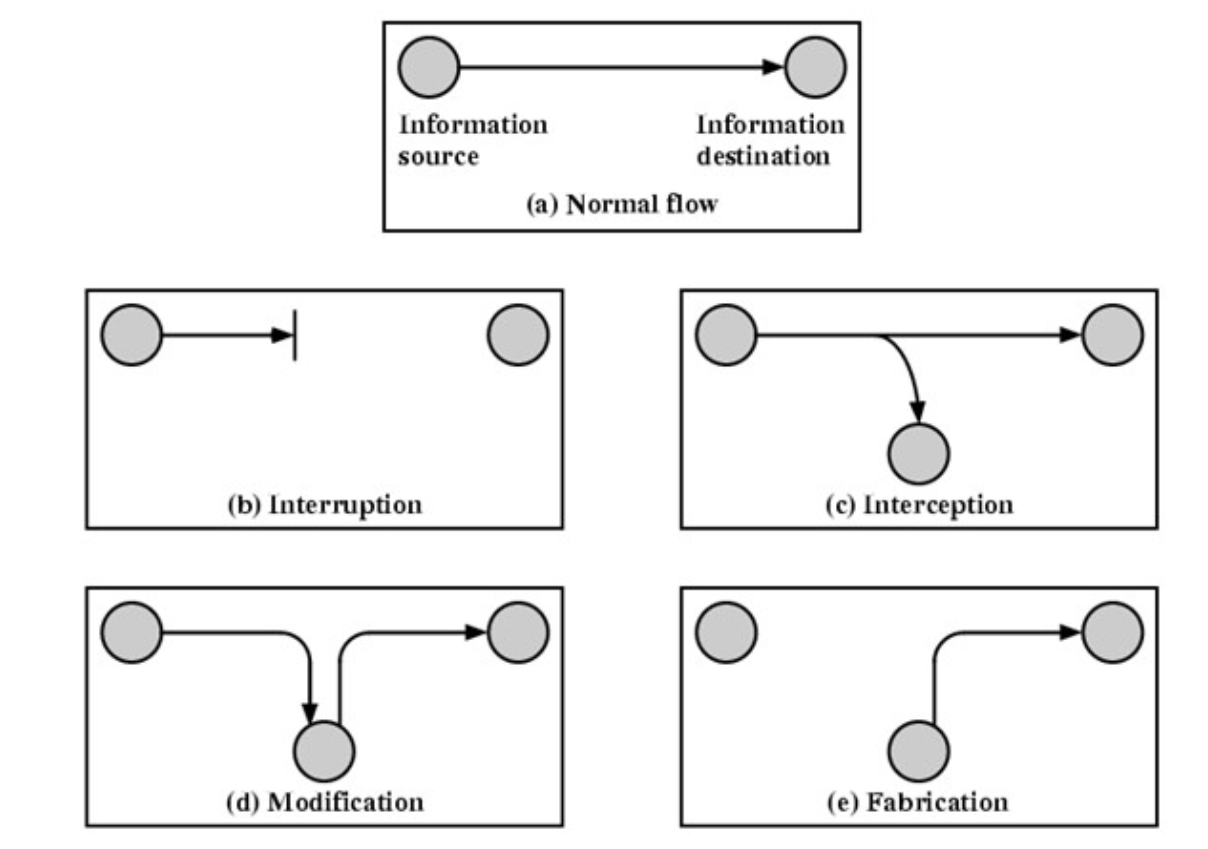
\includegraphics[width=\textwidth]{images/angriffe_pic1.png}
    \caption[Beschriebung für Inhaltsverzeichnis]{Bildbeschreibung} 
    \label{Referenz}
\end{figure} 

\textbf{Unterbrechungen}
\textbf{Abfangen}
\textbf{Modifikation}
\textbf{Fälschung}

Desweiteren gibt es noch eine EInteilung in Passive und aktive Angriffe. 



\section{Anforderungen an verteilte Systeme}


